\section{Question/Answer Database Analysis}\label{sec:unsafe:so}

To complement the analysis of \smu{} usage in practice,
and to answer the questions relative to which features are commonly used ($Q2$),
why they are used ($Q3$),
and if they generate issues or problems ($Q4$),
we search for discussions concerning the usage of \smu{} in \stackoverflow{}.
We cannot rely only on \stackoverflow{} discussion tags:
The topic is rarely discussed,
and the tag \emph{unsafe} is too general.
A more precise analysis of the discussion contents is required to understand if it actually involves \smu{}.
We rely on parsing \emph{island grammars}~\cite{Moon2001a} of structured fragments in natural language artifacts~\cite{Bacc2011f,Ponz2015a} to discover discussions that involve \smu{} from the \stackoverflow{} data dump of March 2015.%
\footnote{\url{https://archive.org/details/stackexchange}}

\subsection{(Island) Parsing \stackoverflow{} Discussions}

Our island grammar parsing approach can be used to discover and analyze specific constructs that reveal the usage of \smu{}.
For example, a discussion could report a code sample using \smu{},
or a user could mention the class (or one of its fields/methods) in an answer to a question concerning some specific problem that the usage of \smu{} can tackle.
The island grammar allows us to identify constructs like stack traces and \java{} code fragments,
including (potentially incomplete) method invocations or mentions inside natural language text.
We do not perform simple identification and extraction,
but we rather model the contents with a Heterogeneous Abstract Syntax Tree (H-AST)~\cite{Ponz2015a}.

\textbf{Identifying Relevant Discussions.}
We identify \stackoverflow{} discussions concerning the \smu{} class by analyzing all the discussions tagged with one of \emph{java}, \emph{scala}, \emph{android}, or \emph{jvm}.
To understand if a discussion concerns \smu{}, we search for
(i) uses of fields or methods exposed by \unsafe{} or
(ii) mentions of the class itself.
We extract discussions where the HAST contains either
\begin{inparaenum}[(i)]
\item a qualified identifier matching  \unsafe{}, \emph{unsafe}, \emph{UNSAFE}, or \smu{};
\item an invocation of a method declared in \smu; or
\item \java{} identifiers, beginning with a lowercase letter and containing a case change (\eg ``fieldOffset''), that respect method naming conventions and match one of the methods declared in \unsafe{}.
\end{inparaenum}

\textbf{Qualified Identifiers.}
Qualified identifiers appear in constructs like import declarations and stack trace lines.
We check that the qualified identifier matches values such as
\unsafe{}, \emph{unsafe}, \emph{UNSAFE}, or the fully-qualified type \smu{}.
In case of match, the post is marked as mentioning the type \unsafe{}.
Moreover, if the last part of the qualified identifier matches the name of one of the \smu{} fields,
we mark the post as mentioning a field of \unsafe{}.

\textbf{Method Invocations.}
Each node matching a method invocation is analyzed to understand if the method name belongs to \smu{}.
We also perform check on the callee to understand if the method invocation is effectively performed on the \unsafe{} class.
We check this information on the callee by applying the same rules used for qualified identifiers.

\textbf{Strict Identifiers.}
We extract identifiers respecting the \java{} naming conventions for methods and that are present in the narrative.
Identifiers beginning with a lowercase letter and containing a case change
(\eg{}, ``fieldOffset'') are considered as method names.
The method name must then match one of the methods declared in \unsafe{}.
We also check qualified identifiers appearing in the narrative and respecting naming convention for classes.
We look for all the occurrences of qualified identifiers composed by three identifiers at least (\eg{}, \smu{}).
Whatever matches this construct is treated as a normal qualified identifier.

\textbf{String Literals.}
We verify that the fully qualified type \smu{} is present in the literal contents.
We also verify that literal matches the string ``theUnsafe''.
This string is a special field name in the \unsafe{} class for the HotSpot VM to get the instance via reflection.

\textbf{Refining Parsing Results.}
The \code{park} method appears at the top of stack traces for idle threads.
Since these occurrences do not represent an interesting usage of \unsafe{},
we therefore removed all discussions where the only usage of \unsafe{} is the \member{park} method occurring in a stack trace.

We collected 20,915 discussions matching at least one of the two criteria,
out of which 560 discussions report only the type \unsafe{},
20,426 contain a method with a name matching the ones of \unsafe{},
and 5 discussions mention a field of \unsafe{}.
However, if the presence of the type \unsafe{} guarantees that the discussion is likely about \smu{},
the lone presence of the method name does not guarantee that.
For example, methods like \code{getInt} and \code{getFloat} can be found in other classes like \code{java.nio.ByteBuffer}.%
\footnote{\url{http://docs.oracle.com/javase/7/docs/api/java/nio/ByteBuffer.html}}.
Neither does the absence of the type in our parsing results guarantee that the discussion does not concern \smu{}.
Indeed, to avoid false positives,
we do not check at parsing time if the lone term ``unsafe'' is mentioned in the natural language parts of a discussion.

After parsing, we consider all discussions with a method name of the class \unsafe{},
and we perform a pure text search for the term ``unsafe''.
Out of 20,426 discussions that mention an \unsafe{} method,
49 discussions also contain the term ``unsafe''.
We manually inspected and verified each discussion,
resorting to 18 discussions effectively reporting a usage of \smu{}.
Thus, our final dataset contains a 560 discussions explicitly using the type \unsafe{},
and 18 discussions reporting the method name only and the term ``unsafe'',
for a total of 578 discussions that effectively concern \smu{}.
Of these ones, 163 questions mention both the type (or the term \emph{unsafe}) and at least one of its methods.


\subsection{Findings on \stackoverflow{} Discussions}

Figure~\ref{fig:unsafe:usage-so} presents an overview of \smu{} method mentions in \stackoverflow{}.
The mentions are presented by distinguishing whether they appear only in the question,
only in the answer, or in both.
The list of methods does not distinguish between overloaded variants.
In fact, people often mention method names without formal or actual parameters.
Thus, in many cases, to understand which is the overloaded alternative one would have to do a manual inspection. 

Most method mentions appear in answers only,
indicating a prevalence of the use of \smu{} as a proposed solution for some task.
In other frequent cases, they are present in both questions and answers.
More rarely, they are present in questions only,
a case that captures a clarification from the user that mostly requires narrative only,
\eg{}, for documentation).
The most mentioned method in \stackoverflow{} discussions is \member{allocateInstance},
followed by \member{getInt}.
The former is often proposed in the replies,
suggesting its use for some particular task,
or it is present in both questions and answer,
discussing a particular task for which the developer is already aware of its possible use.
The most frequently occurring groups of methods are \smugroup{Get} and \smugroup{Off-Heap}.
Moreover, the methods mentioned most in questions are the ones in the \smugroup{Put} group.
Finally, the methods from \smugroup{Fetch \& Add} group are not mentioned in our dataset.

% \clearpage
\begin{figure}[h!]
\centering
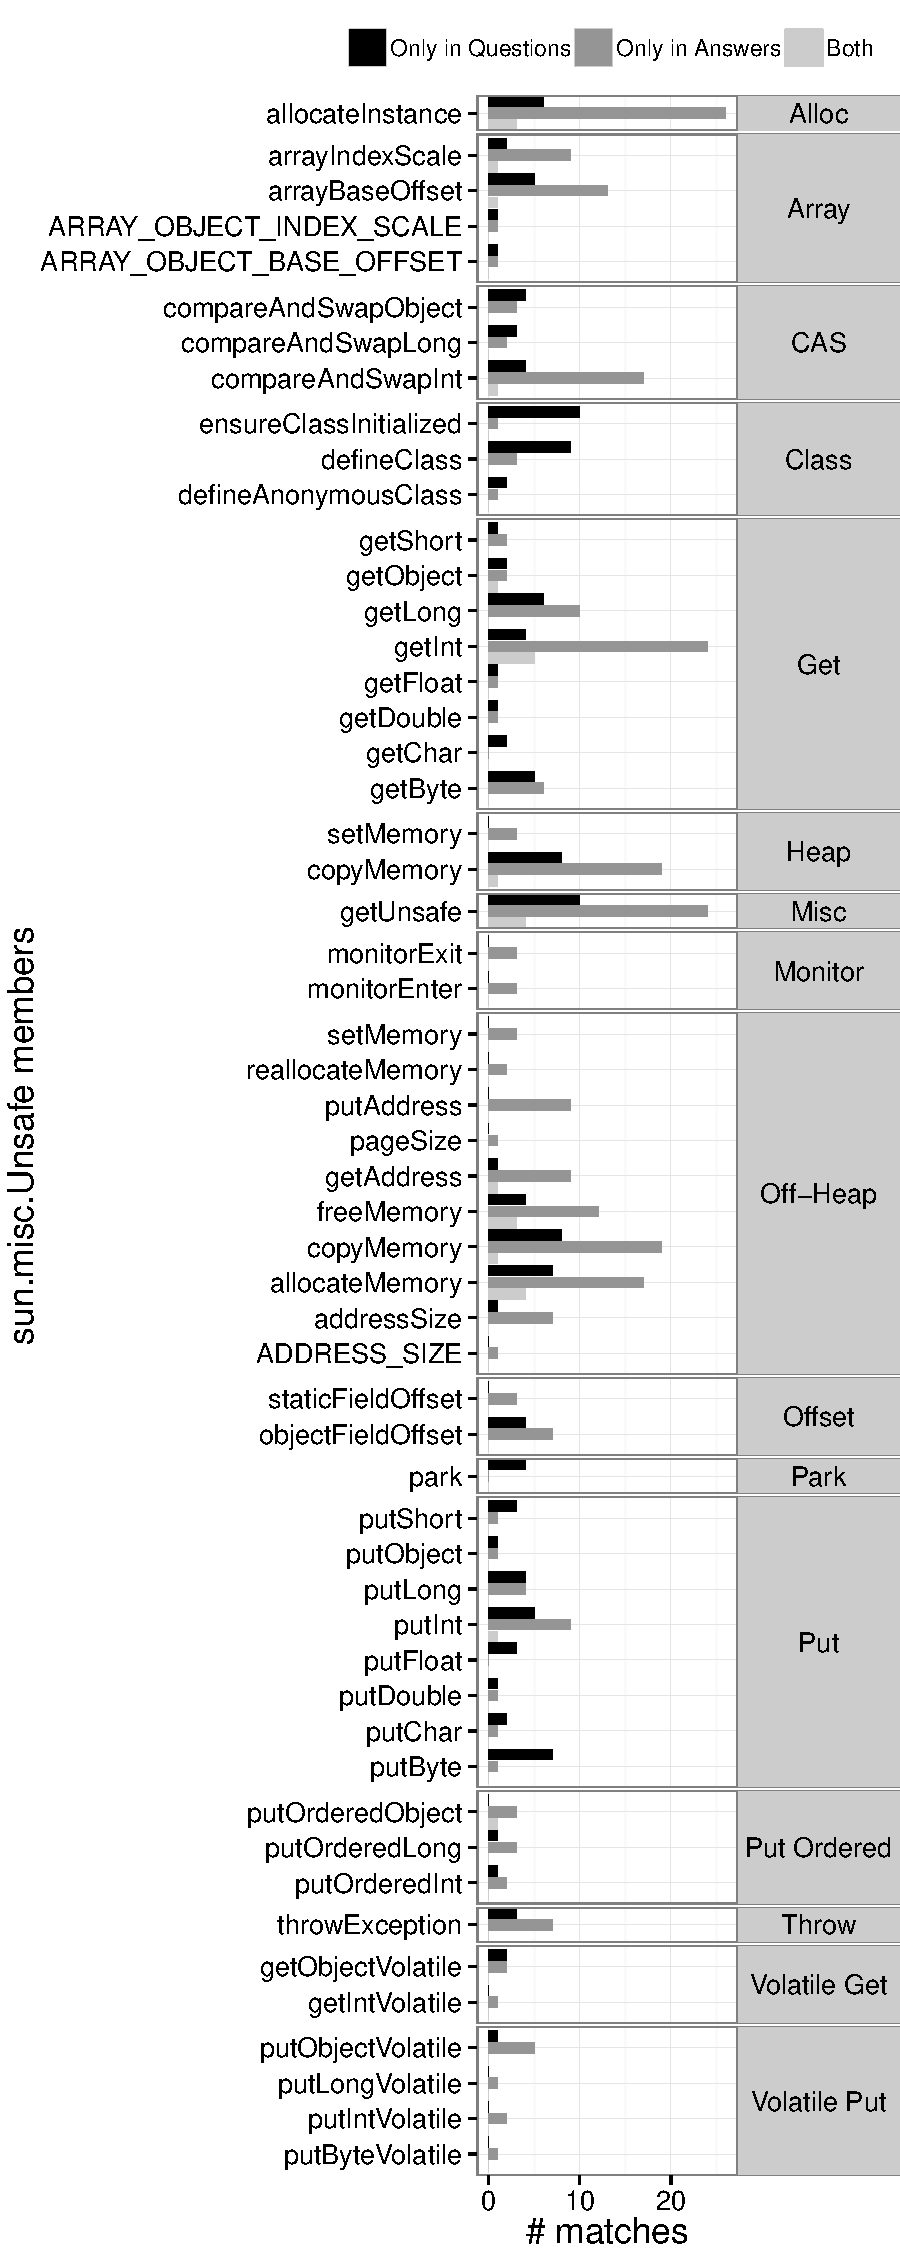
\includegraphics[width=0.54\textwidth]{chapters/unsafe/usage-so}
\caption{\smu{} members mentions on \stackoverflow{}}
\label{fig:unsafe:usage-so}
\end{figure}

{ \bfseries Discussions Archetypes. } 
We manually inspected the resulting discussions to understand how \smu{} is discussed, devising a set of discussion archetypes:

\begin{itemize}
\item\textbf{Lack of documentation.}
\unsafe{} is an undocumented API,
and a primary archetype concerns developers asking the crowd to obtain clarification on usage.
A relatively popular question, entitled ``Using sun.misc.Unsafe in real world'',
asks for typical use cases.%
\footnote{\url{http://stackoverflow.com/questions/5574241}}

\item\textbf{Performance.}
Users coming from unmanaged languages like \c{} and \cpp{} discuss how to avoid the cost of \java{}'s safety checks.
For instance, a user asked for an equivalent method call for \code{memcpy}.%
\footnote{\url{http://stackoverflow.com/questions/6060163}}

\item \textbf{Misdirected uses.}
Developers may propose \unsafe{} for inappropriate purposes.
For example, a post discusses the use of the address to free an object on the \java{} heap.%
\footnote{\url{http://stackoverflow.com/questions/24429777}}
Developers suggested the use of \unsafe{} as a workaround to the \code{Runnable.run()} signature%
\footnote{\url{http://stackoverflow.com/questions/11410042}}
to allow it throwing exceptions.
Overall, the availability of \unsafe{} to developers who do not have a deep understanding of the \jvm{} comes with the risk of misdirected uses.
This risk is not unlike the risk of inappropriately using \code{eval}~\cite{Richards:2011:EML:2032497.2032503} in \javascript{}.

\end{itemize}
